\section{Results}
\subsection{Continuation Discovery and Candidate Redundancy}
Full-203 finds a continuation for 335 of the 432 matched inputs. Of the remaining inputs, 71 have no feasible primary and 26 have feasible primaries but no continuation in the evaluated library. These two groups are excluded from the recall denominator and retained in the computation statistics.

With $K=12$, Cost-12 finds 239 of the 335 available witnesses, whereas Diverse-12 finds 317. Discovery recall therefore increases from 71.34\% to 94.63\%. The paired comparison contains 78 inputs found only by Diverse-12 and none found only by Cost-12. The 23.28 percentage-point difference has a 95\% map-bootstrap interval of [13.27,34.66]. Across the 24 maps, the diversity schedule improves recall on 14 and ties on ten. Figure~\ref{fig:matched} and Table~\ref{tab:matched} summarize discovery, validation work, timing, and primary-cost effects.

The mean continuation work is similar for the two candidate-limited methods: 20,605 steps for Cost-12 and 21,054 for Diverse-12. Full-203 requires 81,388 mean continuation steps. Common primary propagation accounts for approximately 30,592 steps per input. Thus, endpoint coverage substantially increases discovery within the 12-candidate allowance without a comparable increase in mean continuation integration work on this suite.

The diversity schedule also changes which feasible primary is selected. On the 239 inputs where both methods find a witness, its selected cost is equal or higher: the median difference is zero, the mean is 0.514, and the 95th percentile is 1.929. Whenever Cost-12 finds a witness, its selection equals the Full-203 minimum-cost choice; the coverage schedule spends some of its allowance on more distant terminal motions. This tradeoff explains why discovery and immediate task cost should be reported together.

\begin{figure*}[!t]
\centering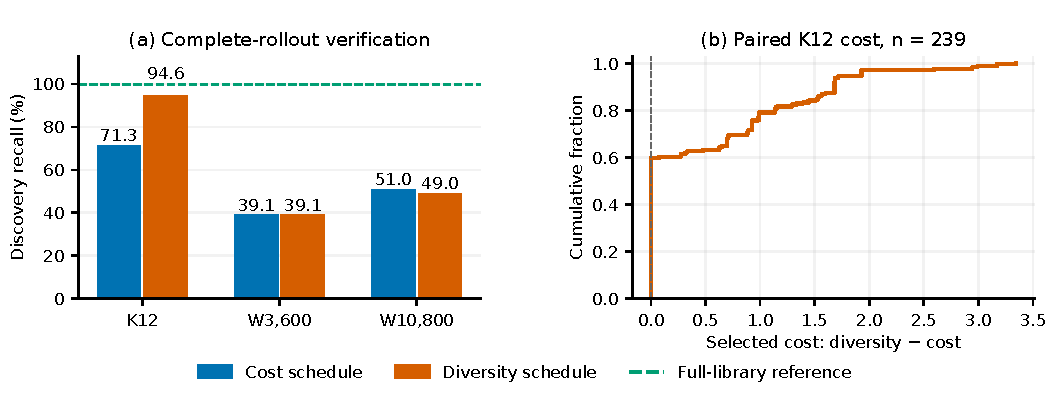
\includegraphics[width=\textwidth]{figures/matched.pdf}
\caption{Matched-input comparison using complete continuation rollouts. Discovery is measured on the 335 Full-203-positive inputs. The cost difference is computed on the 239 inputs verified by both $K=12$ methods.}
\label{fig:matched}
\end{figure*}

\begin{table*}[!t]
\centering\small
\caption{Matched-input discovery and computation with complete continuation rollouts. Each method receives the same 432 states; two timing repeats are merged per state.}
\label{tab:matched}
% Generated by analyze_recovery_v3.py from audited observations.
\begin{tabular}{lrrrrrr}
\toprule
Method & Verified & Recall (\%) & Median (ms) & P95 (ms) & P99 (ms) & Mean backup steps \\
\midrule
Cost, K=12 & 239 & 71.3 & 3.64 & 9.31 & 9.39 & 20605 \\
Diverse, K=12 & 317 & 94.6 & 4.22 & 8.86 & 8.96 & 21054 \\
Full, K=203 & 335 & 100.0 & 3.62 & 41.88 & 52.65 & 81388 \\
Cost, W=3,600 & 131 & 39.1 & 2.80 & 4.33 & 4.34 & 2091 \\
Diverse, W=3,600 & 131 & 39.1 & 2.97 & 4.54 & 4.56 & 2091 \\
Cost, W=10,800 & 171 & 51.0 & 3.23 & 5.09 & 5.62 & 5424 \\
Diverse, W=10,800 & 164 & 49.0 & 3.53 & 5.13 & 5.19 & 5894 \\
\bottomrule
\end{tabular}

\end{table*}

\subsection{Candidate Budgets and Integration Budgets}
Table~\ref{tab:matched} shows that candidate and integration budgets yield different comparisons. At a 3,600-step limit, both schedules discover 131 witnesses, giving 39.10\% recall. At 10,800 steps, the cost schedule finds 171 and the diversity schedule 164. The paired difference is $-2.09$ percentage points, with a 95\% map interval of [$-6.50$,3.07]. The benefit observed at $K=12$ therefore does not carry over to these smaller work limits under complete-rollout validation.

This result follows from the nested structure of the search. Both schedules start with the cheapest feasible primary. A 3,600-step budget can be consumed before all 15 continuation controls of this first endpoint have been tested. Terminal diversity becomes relevant only when enough work remains to reach additional endpoints. Moreover, integrating a continuation after its first constraint violation consumes budget without changing its rejection. The following incremental-rejection experiment addresses this source of computation directly.

\subsection{Incremental Rejection}
Incremental rejection preserves every K12 and Full-203 decision, selected rank, and selected cost across all 432 matched inputs. Repeating the closed-loop matrix also reproduces all 480 outcomes, 27,771 trajectory records, and 27,291 planning decisions exactly; only computation and rejection accounting change. It substantially reduces the work needed to obtain those decisions. Mean continuation integration falls from 20,605 to 6,210 steps for Cost-12, from 21,054 to 2,654 for Diverse-12, and from 81,388 to 13,698 for Full-203. These reductions are 69.86\%, 87.39\%, and 83.17\%, respectively. Figure~\ref{fig:incremental} compares both validators.

The reduction changes the work-limited search. At $W=3{,}600$, incremental cost ordering finds 204 of the 335 reference witnesses, whereas incremental diversity finds 269: recall increases from 60.90\% to 80.30\%. The paired difference is 19.40 percentage points with a 95\% map interval of [6.63,34.66]. At $W=10{,}800$, the corresponding counts are 227 and 317, or 67.76\% and 94.63\%. The difference is 26.87 percentage points [15.00,40.46], with 90 inputs found only by diversity and none found only by cost ordering.

With failed rollouts removed early, the 10,800-step diversity search reaches the same 317 witnesses as the 12-candidate diversity search. This result connects the scheduling and validation components: dispersed terminal endpoints provide useful alternatives only when the validator can reach them within its work allowance. The complete-rollout ablation does not exhibit a diversity advantage at these work limits.

Incremental Diverse-12 has median, P95, and P99 planning times of 2.89, 4.62, and 4.72 ms. Incremental Cost-12 gives 2.74, 6.68, and 6.88 ms, while Full-203 gives 2.74, 11.71, and 12.38 ms. The diversity schedule has a slightly larger median than cost ordering but a shorter upper tail. These timings come from separate runs of the two validator implementations; the exact integration counters provide the direct measure of eliminated numerical work.

\begin{figure*}[!t]
\centering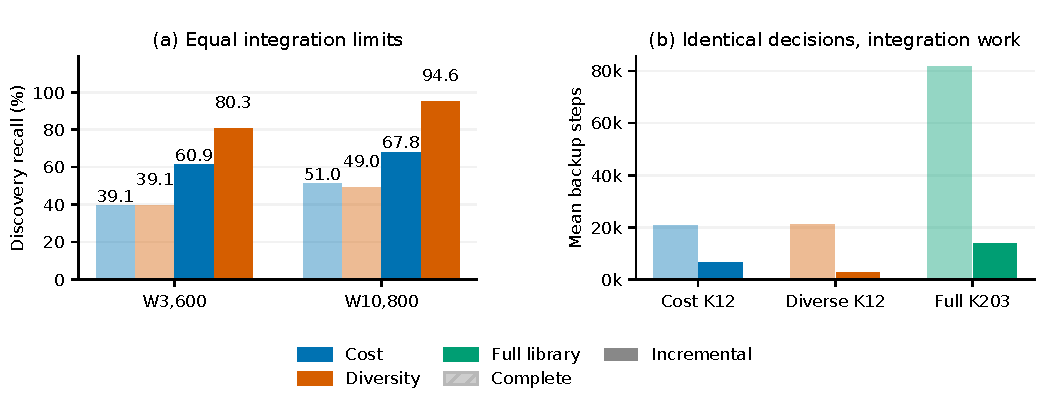
\includegraphics[width=\textwidth]{figures/incremental.pdf}
\caption{Effect of incremental rejection on the same matched inputs. Work-budget comparisons use identical upper limits; consumed work can be smaller after early success. The complete-rollout results are retained to isolate the effect of ending a continuation at its first violated constraint.}
\label{fig:incremental}
\end{figure*}


\subsection{Closed-Loop Task Completion}
Figure~\ref{fig:outcomes} reports all 480 episode outcomes. Aggregated over the four execution conditions, Primary-3 completes 28 of 96 tasks, Primary-6 completes 43, Cost-12 completes 37, Diverse-12 completes 56, and Full-203 completes 67. Diverse-12 gains 19 completions over Cost-12. In the paired comparison, 26 tasks succeed only with diversity and seven only with cost ordering, corresponding to a 19.79 percentage-point difference with a 95\% map-bootstrap interval of [5.21,35.42]. The longer primary-only ablation improves over Primary-3 but remains below Diverse-12 in total completion.

Under nominal RK4 execution, the completion counts are 11, 14, and 20 for Cost-12, Diverse-12, and Full-203. Under parameter mismatch, they are 12, 15, and 20. The crosswind condition is the most demanding: the same methods complete one, seven, and six tasks. A constant lateral wind changes the ground trajectory over the entire prediction horizon, while the planner continues to propagate the nominal air-relative model. Replanning from measured state alone does not compensate for this accumulated prediction error.

The 100 ms delay condition yields 13, 20, and 21 completions for Cost-12, Diverse-12, and Full-203. Some counts exceed those under nominal execution; command holding changes the closed-loop path and the sequence of subsequently generated candidates. Consequently, task completion can vary nonmonotonically with delay in this deterministic suite.

Obstacle-margin incursions occur in five Diverse-12 episodes and none of the Cost-12 episodes; Full-203 incurs two. All five diversity incursions occur under nominal RK4 execution, immediately after a command with a verified continuation. At margin detection, their logged minimum clearances to the uninflated obstacles range from 1.57 to 2.43 m. The planner uses Euler propagation and evaluates feasibility at discrete samples, so a positive model witness can still approach the inflated boundary too closely during execution. Continuation discovery and preservation of geometric margin are consequently distinct performance measures.

\begin{figure*}[!t]
\centering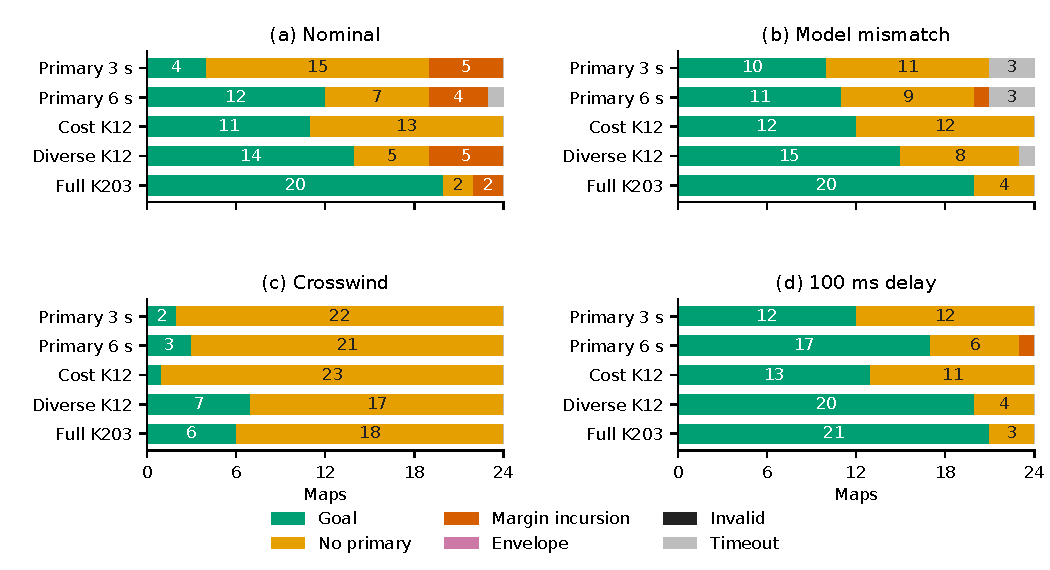
\includegraphics[width=.94\textwidth]{figures/outcomes.pdf}
\caption{Closed-loop outcomes on 24 maps per method and execution condition. Margin incursion denotes entry into inflated obstacle geometry. All methods use the same primary constraints, target tolerance, and 40 s timeout.}
\label{fig:outcomes}
\end{figure*}

Figure~\ref{fig:paths} shows the first seeded map of each family. This fixed selection includes both favorable and unfavorable trajectories. In the cul-de-sac example, Diverse-12 and Full-203 select the early outward turn and complete the route, while the other methods lose feasible primaries near the entrance. In the staggered and spatial examples, the diversity trajectory terminates before completing the task. These examples illustrate how a schedule can improve aggregate continuation discovery while still selecting an unfavorable closed-loop maneuver in an individual map.

\begin{figure*}[!t]
\centering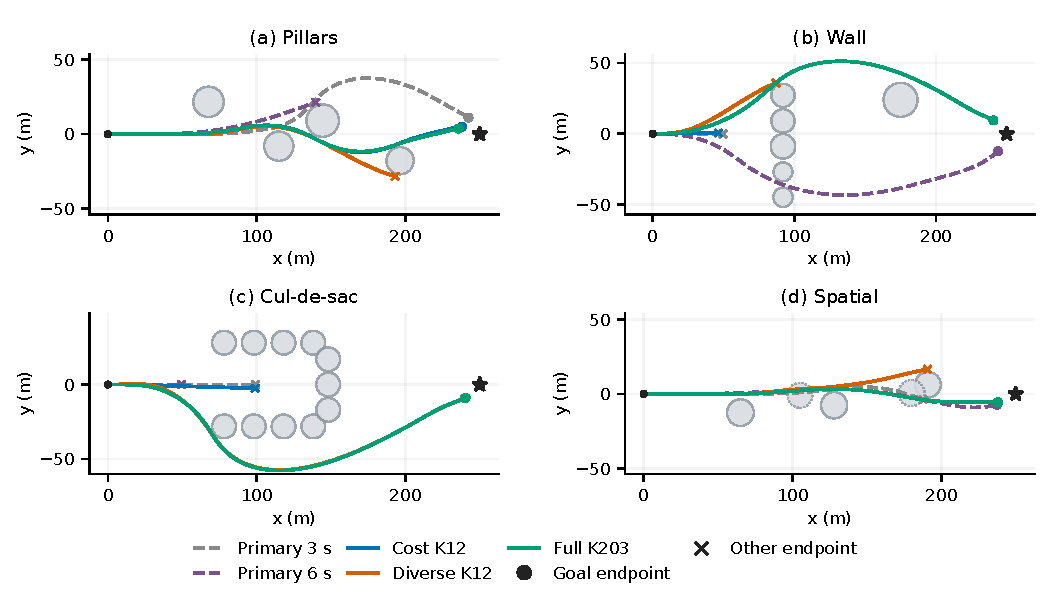
\includegraphics[width=.9\textwidth]{figures/paths.pdf}
\caption{Nominal trajectories for the first seed of each frozen map family. Circles mark successful endpoints and crosses mark other terminations. The spatial-obstacle panel is a horizontal projection; obstacle height and vertical clearance are represented in the simulator.}
\label{fig:paths}
\end{figure*}

\subsection{Observation Range and Revalidated Plan Reuse}
The 17 m/s diagnostic reaches the target at 31.0 s with final horizontal error 13.64 m. It therefore exceeds a 30 s task limit because of the longer executed route. Across 155 planning states, the cache-based planner obtains 78 fresh witnesses and revalidates a remaining plan on 63 further updates; 14 updates execute a feasible primary without a continuation witness.

The matched counterfactual queries distinguish two causes of missing fresh witnesses. With the 120 m boundary, Full-203 fails to find a continuation at 39 visited states; removing the boundary reduces this count to four. Thus, 35 states lose available finite-library witnesses specifically because of the observation restriction. At the same restricted states, Diverse-12 misses 38 witnesses found by Full-203. Removing the boundary reduces this budget-miss count to 15. Figure~\ref{fig:diagnostic} shows how these effects vary along the executed route.

The range effect is consistent with the geometry of a 3 s primary followed by a 6 s continuation: at 17 m/s, a straight nominal traversal covers approximately 153 m, exceeding the 120 m validation radius. Curved trajectories may remain within the sphere, but the constraint changes which terminal maneuvers can receive a witness. Reuse allows a previously verified sequence to continue through some of the resulting gaps in fresh search. It also changes the path, so its task-level effect requires separate evaluation from the scheduling rule.

\begin{figure*}[!t]
\centering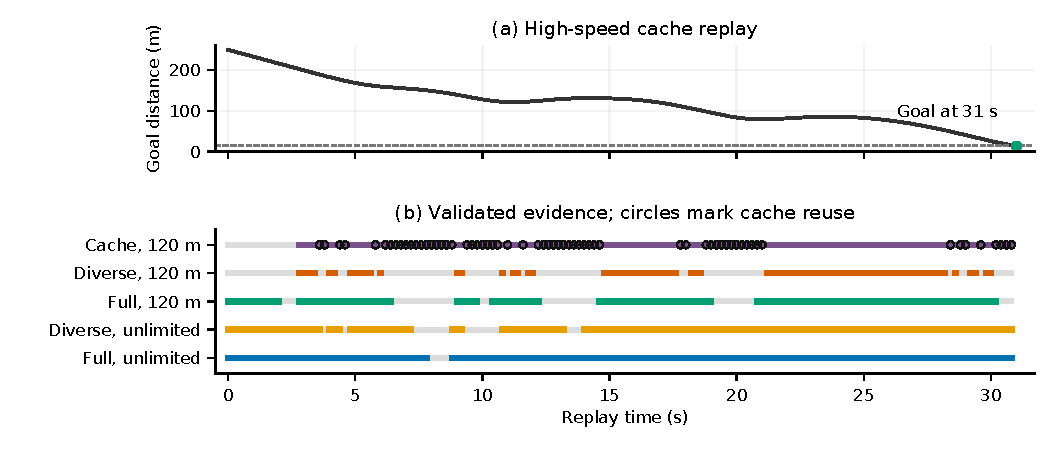
\includegraphics[width=.9\textwidth]{figures/diagnostic.pdf}
\caption{Range-limited diagnostic with same-state counterfactual queries. A cache-reuse marker denotes revalidation of the remaining previously selected sequence; a fresh witness denotes a new primary--continuation pair. All queries use complete-rollout validation.}
\label{fig:diagnostic}
\end{figure*}

\section{Discussion}
The experiments identify two complementary requirements for effective terminal validation. The schedule must reach distinct maneuvers, and the validator must avoid spending its allowance on continuations already known to fail. A candidate-count budget exposes the first requirement; an integration-step budget exposes both. This distinction is relevant to planners that replace explicit candidates with learned proposals as well: a proposal's task score alone does not describe the cost or information value of validating its future motion.

The closed-loop simulations also separate finite continuation feasibility from task completion. A witness establishes a feasible sampled primary--successor pair under the prediction model. It does not impose a periodic terminal maneuver or a recursively invariant terminal set. The remaining failure cases point to two concrete extensions: model-aware clearance margins, especially for wind, and stronger terminal maneuvers that preserve useful flight space beyond one successor. A learned validation schedule could additionally exploit obstacle geometry and the full terminal dynamic state when heading--altitude coverage is insufficient.

The current evidence concerns static generated maps and a point-mass aircraft with actuator dynamics. The principal suite provides full geometry; the observation-radius test is a separate diagnostic, without camera occlusion. The 24-map bootstrap measures variability within this suite. Tests with sensed local maps, a six-degree-of-freedom aircraft model, and real flight would determine how the observed scheduling effects transfer to a deployed system.
